\section{استخراج رابطه با تکنیک نظارت از راه دور با استفاده از دروازه در شبکه عصبی پیچشی تکه‌ای با تاکید بر موجودیت‌ها \cite{gated}}

محتوای جمله و به خصوص موجودیت‌ها تاثیر زیادی در معنای برداشت شده از جمله و کلمه دارند. هایخو ون\LTRfootnote{Haixu Wen}، شین‌هوآ ژو\LTRfootnote{Xinhua Zhu}،
لانفانگ ژنگ\LTRfootnote{Lanfang Zhang} و فی لی\LTRfootnote{Fei Li} تلاش کردند با استفاده از مکانیزم توجه به خود\LTRfootnote{self attension}
بهتر بتوانند محتوای جمله را در معنای کلمه دخیل کنند. آن‌ها برای انجام این کار از شبکه عصبی پیچشی تکه‌ای
و مکانیزم دروازه\LTRfootnote{gate} استفاده کردند.

\begin{figure}[h]
    \centering
    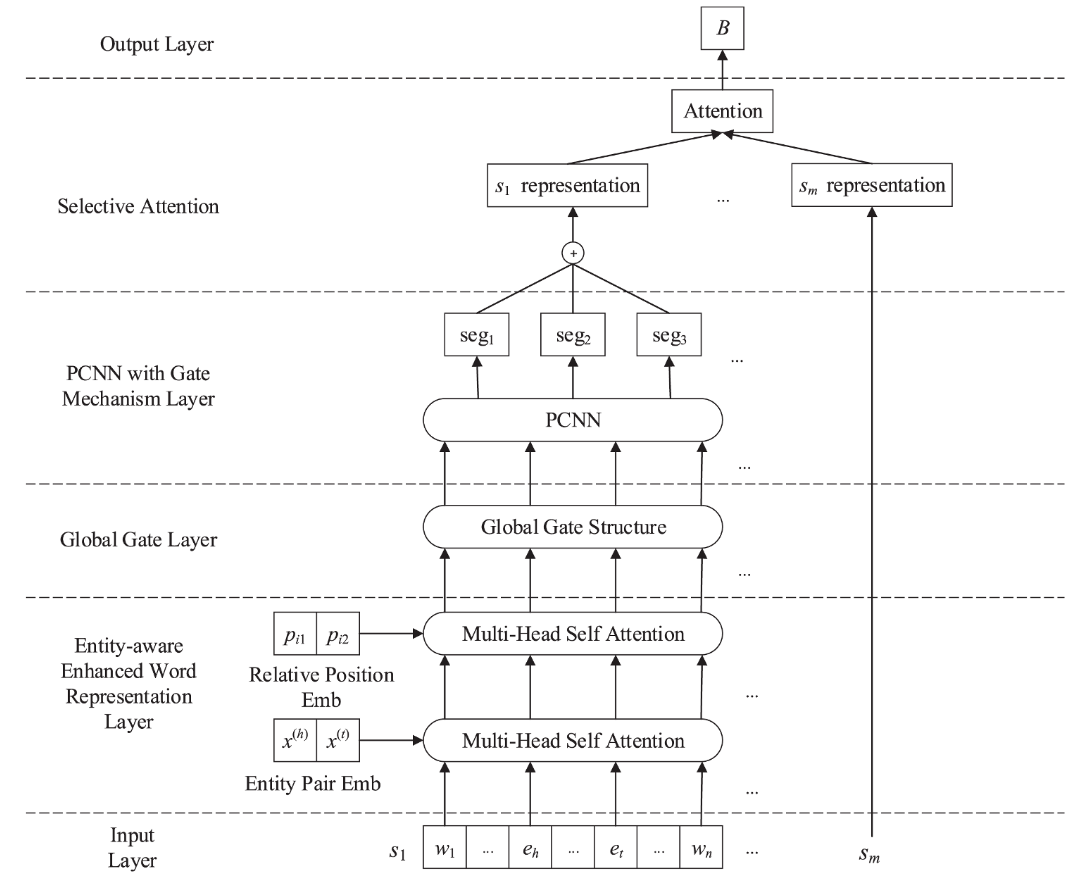
\includegraphics[scale=0.22]{images/gated/architecture.png}
    \caption{معماری شبکه مقاله استخراج رابطه با تکنیک نظارت از راه دور با استفاده از دروازه در شبکه عصبی پیچشی تکه‌ای با تاکید بر موجودیت‌ها}
    \label{gated}
\end{figure}

شکل \ref{gated} خلاصه کار انجام شده توسط ون و همکاران را نشان می‌دهد. در این شبکه ابتدا هر کلمه با استفاده از
مدل \lr{word2vec} به بردار تبدیل می‌شود. در قدم بعدی ترکیب بردار موجودیت‌ها با بردار کلمه
به لایه توجه به خود داده می‌شود تا بازنمایی بهتری برای کلمه با تاکید بر بازنمایی موجودیت‌ها تولید شود. به عبارتی اگر بردار کلمه $i$ام را با $x_i$ و بردار موجودیت اول
را با $e^{h}$ و بردار موجودیت دوم را با $e^{t}$ نمایش دهیم، در این صورت بردار ورودی به لایه توجه به خود برابر خواهد
بود با

\begin{eqnarray}
    [x_i, e^{h}, e^{t}]
\end{eqnarray}

فرض کنیم خروجی لایه توجه به خود در قدم قبلی بردار $x^{h}_i$ باشد. برای پررنگ‌‌‌تر کردن همبستگی بین هر کلمه و
موجودیت‌، بردار $x^{h}_i$ با فاصله مکانی نسبی کلمه تا هر یک از موجودیت‌ها، که آن را با $p_{i,1}$ و
$p_{i,2}$ نشان می‌دهند، ترکیب شده و حاصل مجددا به لایه توجه به خود داده می‌شود. البته این لایه توجه به خود
متفاوت از لایه توجه به خود توضیح داده شده در پاراگراف قبلی است. به عبارتی ورودی لایه توجه به
خود در این حالت برابر خواهد بود با

\begin{eqnarray}
    [x^{h}_i, p_{i,1}, p_{i,2}]
\end{eqnarray}

خروجی قسمت قبل برای هر کلمه را با علامت $x^{ep}_i$ نمایش می‌دهیم. در گام بعدی بردار حاصل شده به لایه دروازه سراسری\LTRfootnote{global gate}
داده می‌شود. ساختار این بخش در شکل \ref{gate_structure} مشاهده می‌شود. در لایه دروازه سراسری ابتدا بردار میانگین یک جمله بر اساس
بردار‌های $x^{ep}_i$ محاسبه می‌شود. برای محاسبه میزان همبستگی بردار میانگین با هر یک از بردار‌های کلمات، حاصل ضرب نقطه‌ای
بین بردار میانگین و بردار کلمه ($x^{ep}_i$) محاسبه می‌شود. در ادامه بردار حاصل شده از حاصل‌ضرب نقطه‌ای با عبور از یک لایه
متراکم حالت ضریب به خود پیدا می‌کند. بردار‌های بازنمایی نهایی با ضرب این مقادیر ضریب در هر یک از بردار‌ها محاسبه می‌شود.
به بیان ریاضی

\begin{eqnarray}
    \bar{x} & = & \frac{1}{n} \sum_{i}^{n} x^{ep}_i \\
    g_i & = & \sigma(W^g (x^{ep}_i \odot \bar{x}) + b^g) \\
    x^{g}_i & = & x^{ep}_i \odot g_i
\end{eqnarray}

\begin{figure}[h]
    \centering
    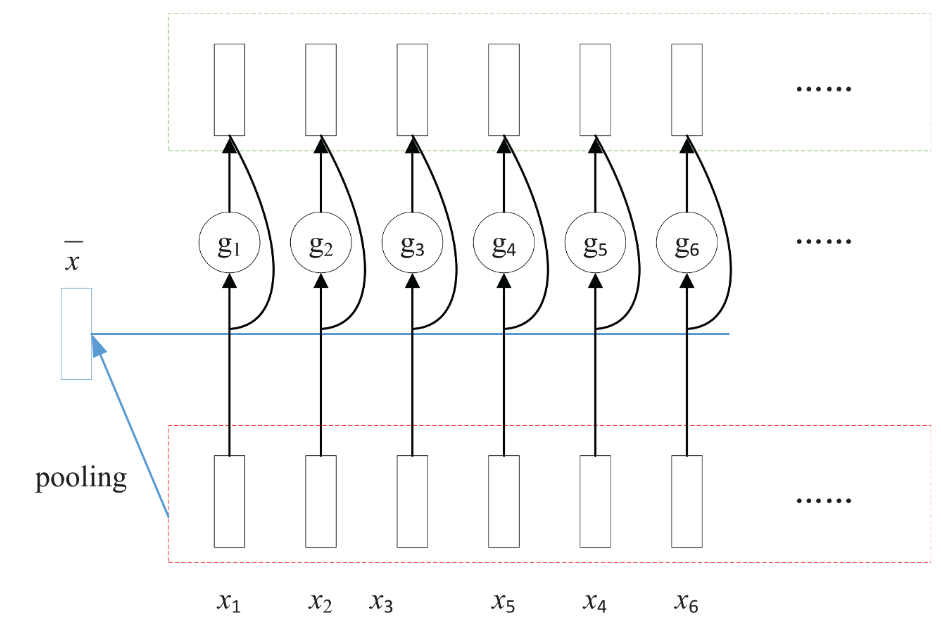
\includegraphics[scale=0.2]{images/gated/gate.png}
    \caption{ساختار قسمت دروازه سراسری}
    \label{gate_structure}
\end{figure}

بردار‌های حاصل شده از لایه دروازه سراسری ($x^{g}_i$) به شبکه \lr{PCNN} داده می‌شود. شبکه \lr{PCNN}
برای سه قسمت جمله بازنمایی متفاوتی را ارائه
می‌کند. این بازنمایی‌ها در ادامه مشابه دروازه سراسری از یک لایه متراکم عبور داده شده و وزن‌های حاصل شده در آن‌ها ضرب می‌شود.
به عبارت ریاضی اگر فرض کنیم خروجی شبکه \lr{PCNN} برابر $[q_{i,1}, q_{i,2}, q_{i,3}]$ باشد، در این صورت خواهیم داشت:

\begin{eqnarray}
    g_{i, seg} & = & \sigma(W^sq_{i,seg} + b^s) \\
    P_{i,seg} & = & g_{i,seg} \odot q_{i,seg} \\
    s^{i}  & = & \tanh([P_{i,1}; P_{i,2}, P_{i,3}])
\end{eqnarray}

بردار $s$ بردار بازنمایی نهایی از یک جمله در این روش است. در این مقاله برای نادیده گرفتن جملات نویزی از وزن‌دهی
جملات یک دسته استفاده می‌شود. بیان ریاضی این قسمت به صورت زیر انجام می‌شود.

\begin{eqnarray}
    B = \sum_{i} \alpha_i s_i \\
    \alpha_i = \frac{\exp(s_iAv_r)}{\sum_{j} \exp(s_jAv_r)}
\end{eqnarray}

بردار $B$ برای آموزش مدل و تعیین برچسب نمونه در هنگام آزمون استفاده می‌شود.


